\documentclass[11pt]{charter}
\usepackage{enumitem}
\usepackage{pdflscape}
\usepackage{multirow}
\usepackage[table,xcdraw]{xcolor}
% El títulos de la memoria, se usa en la carátula y se puede usar el cualquier lugar del documento con el comando \ttitle
\titulo{Implementación de un nodo sensor LoRa para monitoreo de maquinaria} 

% Nombre del posgrado, se usa en la carátula y se puede usar el cualquier lugar del documento con el comando \degreename
\posgrado{Carrera de Especialización en Sistemas Embebidos} 
%\posgrado{Carrera de Especialización en Internet de las Cosas} 
%\posgrado{Carrera de Especialización en Intelegencia Artificial}
%\posgrado{Maestría en Sistemas Embebidos} 
%\posgrado{Maestría en Internet de las cosas}

% Tu nombre, se puede usar el cualquier lugar del documento con el comando \authorname
\autor{Pablo Aguirre} 

% El nombre del director y co-director, se puede usar el cualquier lugar del documento con el comando \supname y \cosupname y \pertesupname y \pertecosupname
\director{Marcelo Pistarelli}
\pertenenciaDirector{UNR} 
% FIXME:NO IMPLEMENTADO EL CODIRECTOR ni su pertenencia
\codirector{} % si queda vacio no se deberíá incluir 
\pertenenciaCoDirector{}

% Nombre del cliente, quien va a aprobar los resultados del proyecto, se puede usar con el comando \clientename y \empclientename
\cliente{Alejandro Minniti}
\empresaCliente{GENROD S.A.}

% Nombre y pertenencia de los jurados, se pueden usar el cualquier lugar del documento con el comando \jurunoname, \jurdosname y \jurtresname y \perteunoname, \pertedosname y \pertetresname.
\juradoUno{Nombre y Apellido (1)}
\pertenenciaJurUno{pertenencia (1)} 
\juradoDos{Nombre y Apellido (2)}
\pertenenciaJurDos{pertenencia (2)}
\juradoTres{Nombre y Apellido (3)}
\pertenenciaJurTres{pertenencia (3)}
 
\fechaINICIO{22 de junio de 2020}		%Fecha de inicio de la cursada de GdP \fechaInicioName
\fechaFINALPlanificacion{22 de Agosto de 2020} 	%Fecha de final de cursada de GdP
\fechaFINALTrabajo{22 de diciembre de 2020}		%Fecha de defensa pública del trabajo final


\begin{document}

\maketitle
\thispagestyle{empty}
\pagebreak


\thispagestyle{empty}
{\setlength{\parskip}{0pt}
\tableofcontents{}
}
\pagebreak


\section{Registros de cambios}
\label{sec:registro}


\begin{table}[ht]
\label{tab:registro}
\centering
\begin{tabularx}{\linewidth}{@{}|c|X|c|@{}}
\hline
\rowcolor[HTML]{C0C0C0} 
Revisión & \multicolumn{1}{c|}{\cellcolor[HTML]{C0C0C0}Detalles de los cambios realizados} & Fecha      \\ \hline
1.0      & Creación del documento                                          & 10/08/2020 \\ \hline
1.1 	 & Creación capítulos 1-11										   & 10/08/2020 \\ \hline
\end{tabularx}
\end{table}

\pagebreak



\section{Acta de constitución del proyecto}
\label{sec:acta}

\begin{flushright}
Buenos Aires, \fechaInicioName
\end{flushright}

\vspace{2cm}

Por medio de la presente se acuerda con el Ing. \authorname\hspace{1px} que su Trabajo Final de la \degreename\hspace{1px} se titulará ``\ttitle'', consistirá esencialmente en el prototipo preliminar de un sistema de control de variables de producción, y tendrá un presupuesto preliminar estimado de 600 hs de trabajo y \textcolor{red}{\$XXX}, con fecha de inicio \fechaInicioName\hspace{1px} y fecha de presentación pública \fechaFinalName.

Se adjunta a esta acta la planificación inicial.

\vfill

% Esta parte se construye sola con la información que hayan cargado en el preámbulo del documento y no debe modificarla
\begin{table}[ht]
\centering
\begin{tabular}{ccc}
\begin{tabular}[c]{@{}c@{}}Ariel Lutenberg \\ Director posgrado FIUBA\end{tabular} &  & \begin{tabular}[c]{@{}c@{}}\clientename \\ \empclientename \end{tabular} \vspace{2.5cm} \\ 
\multicolumn{3}{c}{\begin{tabular}[c]{@{}c@{}} \supname \\ Director del Trabajo Final\end{tabular}} \vspace{2.5cm} \\
\begin{tabular}[c]{@{}c@{}}\jurunoname \\ Jurado del Trabajo Final\end{tabular}     &  & \begin{tabular}[c]{@{}c@{}}\jurdosname\\ Jurado del Trabajo Final\end{tabular}  \vspace{2.5cm}  \\
\multicolumn{3}{c}{\begin{tabular}[c]{@{}c@{}} \jurtresname\\ Jurado del Trabajo Final\end{tabular}} \vspace{.5cm}                                                                     
\end{tabular}
\end{table}




\section{Descripción técnica-conceptual del proyecto a realizar}
\label{sec:descripcion}

El IIoT (\textit{Industrial Internet of Things}) consiste en maquinaria conectada a Internet y en avanzadas plataformas de análisis que procesan los datos que se producen. Los dispositivos IIoT van desde diminutos sensores ambientales hasta complejos robots industriales. Si bien la palabra ``industrial" puede referirse a almacenes, astilleros y fábricas, las tecnologías IIoT son muy prometedoras para una amplia gama de sectores industriales, como la agricultura, la sanidad, los servicios financieros, el comercio minorista y la publicidad.

Los sensores forman parte de una variedad de roles en la industria moderna. Además de proveer datos para el control de procesos, asisten en la evaluación de calidad, monitoreo de productos, y hasta seguridad del personal. La llegada del software analítico basado en la nube en conjunto con inteligencia artificial también permitió el uso de datos suministrados por sensores para bajar costos de producción mediante optimización y mantenimiento predictivo.
Para servir estos propósitos, existe una amplia variedad de tipos de sensores disponible, con versiones nuevas y mejoradas llegando de manera continua. En la Figura \ref{fig:sensores} se muestran los principales tipos de sensores utilizados en la actualidad.

\vspace{25px}

\begin{figure}[htpb]
\centering 
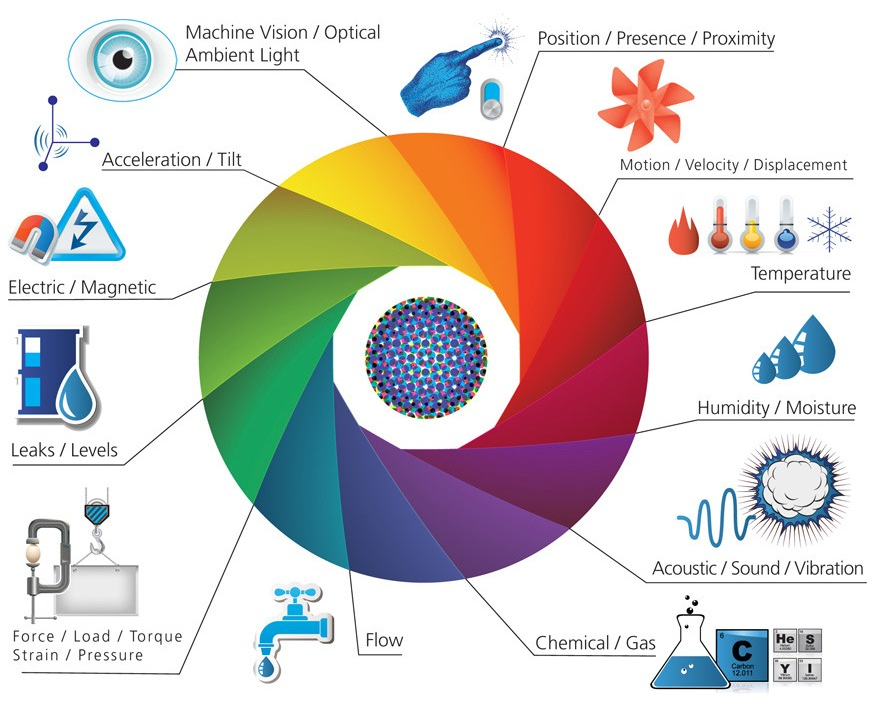
\includegraphics[width=.7\textwidth]{./Figuras/sensores.png}
\caption{Principales tipos de sensores}
\label{fig:sensores}
\end{figure}

\vspace{25px}

GENROD S.A. es una empresa con fábrica propia de gabinetería y tubos dotada con maquinaria de última generación que posee sensores implementados de manera nativa para su control.
Además también se utilizan máquinas que, si bien son perfectamente funcionales, carecen de esta capacidad de control que podría ser de suma utilidad para su monitoreo, pudiendo llevar a su optimización y mejora de productividad. Es por esto que la empresa decidió que sería provechoso poder agregar esta funcionalidad a algunas de sus máquinas.
Existen soluciones en el mercado compuestas de distintos sensores, un gateway que recolecta información de estos y una plataforma de software que recopila y muestra los datos obtenidos que podrían solucionar la inquietud de la empresa. Sin embargo la empresa optó por invertir en el desarrollo de tecnología propia para poder obtener autonomía con soluciones personalizadas y de menor costo, junto con mayor control y entendimiento de ellas.

Como primer paso para lograr esta visión se propuso el presente proyecto consistente en la implementación de un enlace LoRa mediante el cual un extremo recopilará datos de sensores y los enviará al otro extremo que se encargará de recibir estos datos y almacenarlos en una base de datos en una computadora, en la que se podrá obtener una visualización clara de los datos almacenados.
Se optó por utilizar la tecnología LoRa por su capacidad para implementar soluciones de largo alcance (las instalaciones en las que se aplicará tienen alrededor de 20000 $m^2$ y se prevé una expansión) y su idoneidad para enviar datos de telemetría y sensores, con bajo consumo de energía y ancho de banda. Además el hecho de ser un enlace inalámbrico implica menores costos de instalación y materiales que una solución cableada.

El proyecto planteado se presenta en la Figura \ref{fig:diagBloques}. En ella se pueden apreciar los nodos transmisor y receptor. El nodo transmisor tendrá la capacidad de adquirir información de uno o más sensores y la transmitirá mediante un enlace LoRa al nodo receptor, quien se encargará de recibir esta información y transmitirla a una computadora Raspberry Pi, donde será almacenada y podrá ser visualizada con una interfaz gráfica. Los nodos serán implementados con placas de desarrollo suministradas por la empresa.

\vspace{25px}

\begin{figure}[htpb]
\centering 
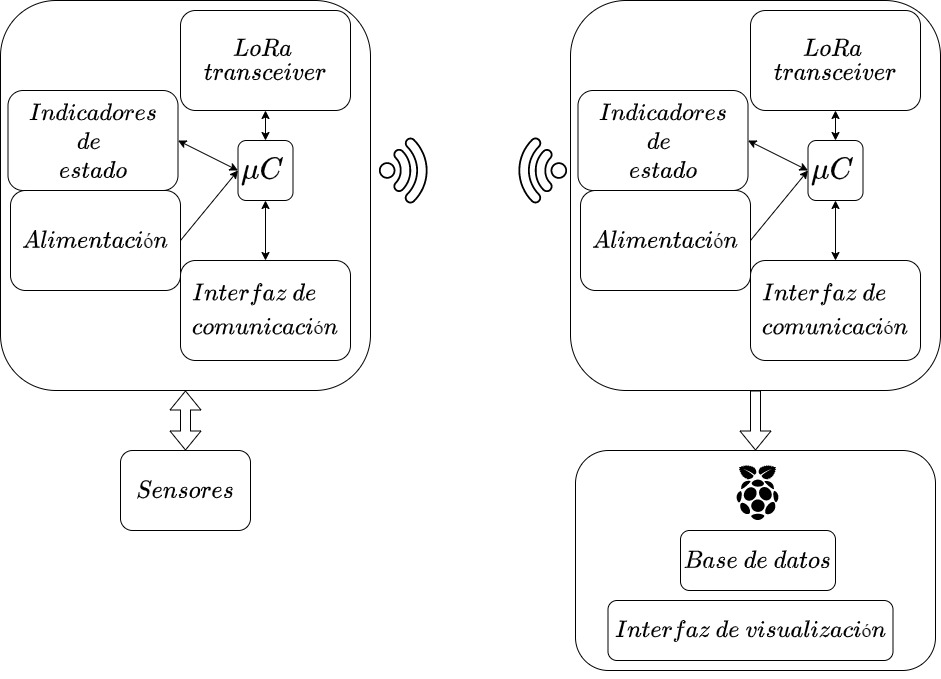
\includegraphics[width=.7\textwidth]{./Figuras/DiagDeBloques.jpg}
\caption{Diagrama en bloques del sistema}
\label{fig:diagBloques}
\end{figure}

\vspace{25px}

Dentro de cada nodo se distinguen los siguientes módulos:
\begin{itemize}
\item[•] \textbf{Microcontrolador:} es el encargado de controlar las operaciones realizadas por los nodos. El microcontrolador presente en las placas de desarrollo es el STM32L072CZ.
\item[•] \textbf{LoRa Transceiver:} módulo encargado de la comunicación LoRa. En la placa de desarrollo el módulo presente es el SX1276.
\item[•] \textbf{Alimentación:} módulo encargado de la alimentación del nodo. En la placa de desarrollo la alimentación puede ser a través de baterías o una entrada micro USB.
\item[•] \textbf{Indicadores de estado:} serán luces LED que indiquen de manera visual el estado del nodo (batería, errores de comunicación, transmisión de datos).
\end{itemize}




\section{Identificación y análisis de los interesados}
\label{sec:interesados}

\begin{table}[ht]
%\caption{Identificación de los interesados}
%\label{tab:interesados}
\begin{tabularx}{\linewidth}{@{}|l|X|X|l|@{}}
\hline
\rowcolor[HTML]{C0C0C0} 
Rol           & Nombre y Apellido & Organización 	& Puesto 	\\ \hline
Cliente       & \clientename      &\empclientename	& Desarrollador	\\ \hline
Responsable   & \authorname       & FIUBA        	& Alumno 	\\ \hline
Orientador    & \supname	      & \pertesupname 	& Director	Trabajo final \\ \hline
Usuario final &    -              &  GENROD S.A.   	& Análisis de datos	\\ \hline
\end{tabularx}
\end{table}


\section{1. Propósito del proyecto}
\label{sec:proposito}

El propósito de este proyecto es desarrollar un prototipo de sistema capaz de comunicar información recibida de sensores colocados en una máquina de la fábrica a través de un enlace LoRa a una computadora, donde será almacenada y podrá ser visualizada.

En un plano más general el propósito de este proyecto es comenzar a generar conocimiento en los temas de sensores, programación de microcontroladores y comunicación LoRa para poder aplicarlo en proyectos futuros en busca de conseguir una fábrica más eficiente y controlada.

\section{2. Alcance del proyecto}
\label{sec:alcance}

El presente proyecto incluirá diseño y creación de software para la implementación de un prototipo de sistema de monitoreo de maquinaria. Dicho sistema está comprendido por un par de nodos de transmisión y recepción de radiofrecuencia utilizando tecnología LoRa. Un nodo permitirá la lectura y transmisión de datos medidos por sensores mediante la implementación de interfaces de comunicación entre estos y el sistema embebido. Otro nodo recibirá la información transmitida de manera inalámbrica y la transferirá a una Raspberry Pi, donde será almacenada a una base de datos y podrá ser visualizada. La implementación a nivel hardware de los nodos se realizará con placas de desarrollo provistas por el cliente.

El proyecto incluye:
\begin{itemize}
\item[•] Diseño del firmware de los nodos.
\item[•] Implementación del firmware de los nodos.
\item[•] Implementación del software encargado de almacenar los datos en una base de datos.
\item[•] Implementación de una herramienta de visualización de los datos adquiridos.
\end{itemize}

El proyecto no incluye:
\begin{itemize}
\item[•] Diseño de hardware.
\item[•] Implementación de una red de nodos.
\end{itemize}


\section{3. Supuestos del proyecto}
\label{sec:supuestos}

Para el desarrollo del presente proyecto se supone que:

\begin{itemize}
\item la empresa cliente proveerá los kits de desarrollo B-L072Z-LRWAN1 de ST.
\item la empresa cliente se hará cargo de la compra de sensores para la adquisición de datos a ser transmitidos por el nodo transmisor.
\item se podrán realizar pruebas dentro de la fábrica.
\item serán respetados los tiempos de trabajo asignados al proyecto durante la etapa de planificación.
\end{itemize}

\section{4. Requerimientos}
\label{sec:requerimientos}

\begin{enumerate}
\item Requerimientos funcionales:
	\begin{enumerate}
	\item Nodo transmisor
		\begin{enumerate}[label*=\arabic*.]
		\item El nodo deberá ser capaz de realizar la lectura de diversos sensores.
		\item El nodo deberá transmitir información de los sensores conectados de manera periódica.
		\item La transmisión de datos deberá ser implementada utilizando LoRa.
		\item La alimentación debe ser implementada mediante baterías AAA.
		\item La nodo deberá tener un sleep-mode configurable para administrar la duración de la batería.
		\item El nodo deberá informar de manera visual cuando tenga poca batería.
		\item El nivel bajo de batería deberá ser informado al nodo receptor.
		\item El nodo deberá informar de manera visual cuando realice una transmisión.
		\end{enumerate}
	\item Nodo receptor
		\begin{enumerate}[label*=\arabic*.]
		\item El nodo deberá recibir información de manera inalámbrica utilizando LoRa.
		\item El nodo deberá informar de manera visual cuando reciba datos.
		\item El nodo deberá reenviar la información recibida hacia la PC utilizada para el almacenamiento de datos.
		\end{enumerate}
	\item Software de manejo de datos
		\begin{enumerate}[label*=\arabic*.]
		\item La información recibida del nodo receptor deberá ser almacenada en una base de datos.
		\item La herramienta de visualización deberá permitir ver más de una variable a la vez.
		\item La herramienta de visualización deberá permitir configurar el span de tiempo que se quiere ver.
		\end{enumerate}
	\end{enumerate}
\item Requerimientos no funcionales
	\begin{enumerate}
	\item Documentación
		\begin{enumerate}[label*=\arabic*.]
		\item Se deberá elaborar un informe de avance del proyecto.
		\item Se deberá elaborar la documentación del firmware desarrollado.
		\item Se deberá elaborar documentación del uso del sistema.
		\end{enumerate}
	\item Testing
		\begin{enumerate}[label*=\arabic*.]
		\item Deberán realizarse pruebas de funcionamiento del sistema antes de su entrega.
		\end{enumerate}
	\end{enumerate}
\end{enumerate}


\section{Historias de usuarios (\textit{Product backlog})}
\label{sec:backlog}

\begin{consigna}{red}
Descripción: En esta sección se deben incluir las historias de usuarios y su ponderación (\textit{history points}). Recordar que las historias de usuarios son descripciones cortas y simples de una característica contada desde la perspectiva de la persona que desea la nueva capacidad, generalmente un usuario o cliente del sistema. La ponderación es un número entero que representa el tamaño de la historia comparada con otras historias de similar tipo.
\end{consigna}

\section{5. Entregables principales del proyecto}
\label{sec:entregables}

Los entregables del proyecto son:
 
\begin{itemize}
\item Firmware nodo transmisor.
\item Firmware nodo receptor.
\item Interfaz de visualización.
\item Documentación del sistema.
\item Informe final.

\end{itemize}

\newpage

\section{6. Desglose del trabajo en tareas}
\label{sec:wbs}
\begin{enumerate}
\item Gestión 																	\hfill \textbf{190 hs}
	\begin{enumerate}
	\item Planificación del proyecto 											\hfill 15
	\item Redacción del informe de avance 										\hfill 25
	\item Redacción documentación nodo transmisor 								\hfill 20
	\item Redacción documentación nodo receptor									\hfill 20
	\item Redacción manual de uso del sistema									\hfill 30
	\item Redacción del informe final 											\hfill 60
	\item Redacción de la presentación final									\hfill 20
	\end{enumerate}
\item Análisis e investigación													\hfill \textbf{70 hs}
	\begin{enumerate}
	\item Búsqueda de información sobre programación de microcontroladores		\hfill 30
	\item Búsqueda de información LoRa											\hfill 20
	\item Búsqueda de información sobre interfaces de visualización				\hfill 20	
	\end{enumerate}
\item Desarrollo de software													\hfill \textbf{230 hs}
	\begin{enumerate}
	\item Selección y configuración del entorno de diseño						\hfill 10
	\item Diseño de arquitectura de firmware de los nodos						\hfill 40
	\item Desarrollo rutinas de lectura y transmisión de datos					\hfill 30
	\item Desarrollo rutinas de control de estado del nodo						\hfill 30
	\item Integración de firmware propio con firmware del módulo de transmisión	\hfill 30
	\item Diseño de arquitectura de software de visualización					\hfill 20
	\item Desarrollo software de adquisición y visualización de datos			\hfill 40
	\item Diseño de detalle														\hfill 30
	\end{enumerate}
\item Testing																	\hfill \textbf{140 hs}
	\begin{enumerate}
	\item Pruebas de firmware de nodo transmisor								\hfill 20
	\item Pruebas de firmware de nodo receptor									\hfill 20
	\item Pruebas de software de adquisición y visualización					\hfill 10
	\item Pruebas de comunicación												\hfill 20
	\item Pruebas de sistema completo											\hfill 30
	\item Corrección de errores													\hfill 40
	\end{enumerate}
\end{enumerate}

Cantidad total de horas: 630 hs

\newpage 
\section{7. Diagrama de Activity On Node}
\label{sec:AoN}

En la Figura \ref{fig:AoN} se muestra el diagrama de \textit{Activity on Node} del proyecto. La unidad de tiempo está expresada en horas.
Se puede observar que existen dos caminos críticos de igual longitud. Estos se encuentran marcados en la figura con un trazo de línea más grueso.
\begin{figure}[htpb]
\centering 
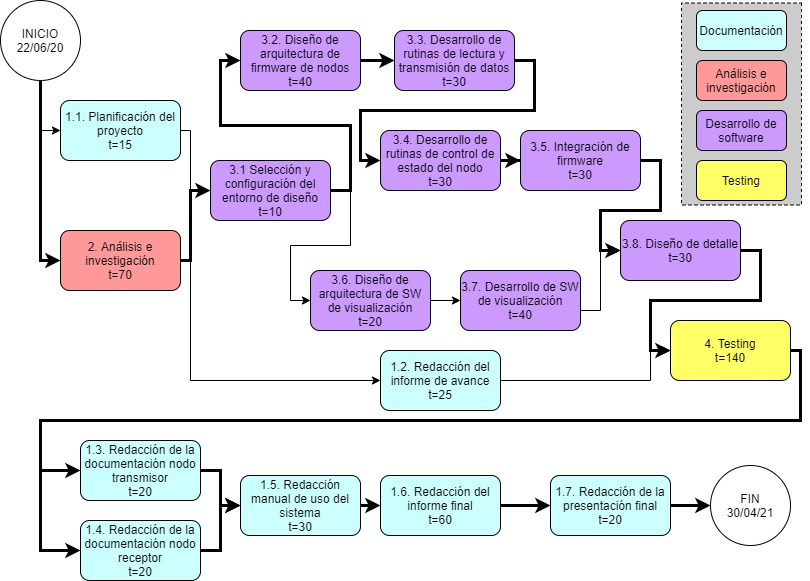
\includegraphics[width=.8\textwidth]{./Figuras/AON.jpg}
\caption{Diagrama en \textit{Activity on Node}}
\label{fig:AoN}
\end{figure}




\section{8. Diagrama de Gantt}
\label{sec:gantt}

El diagrama de Gantt del proyecto se presenta en la Figura \ref{fig:Gantt}. En el mismo se pueden apreciar las fechas de inicio y finalización de cada tarea, así como también sus dependencias.

\begin{landscape}
\begin{figure}[htpb]
\centering 
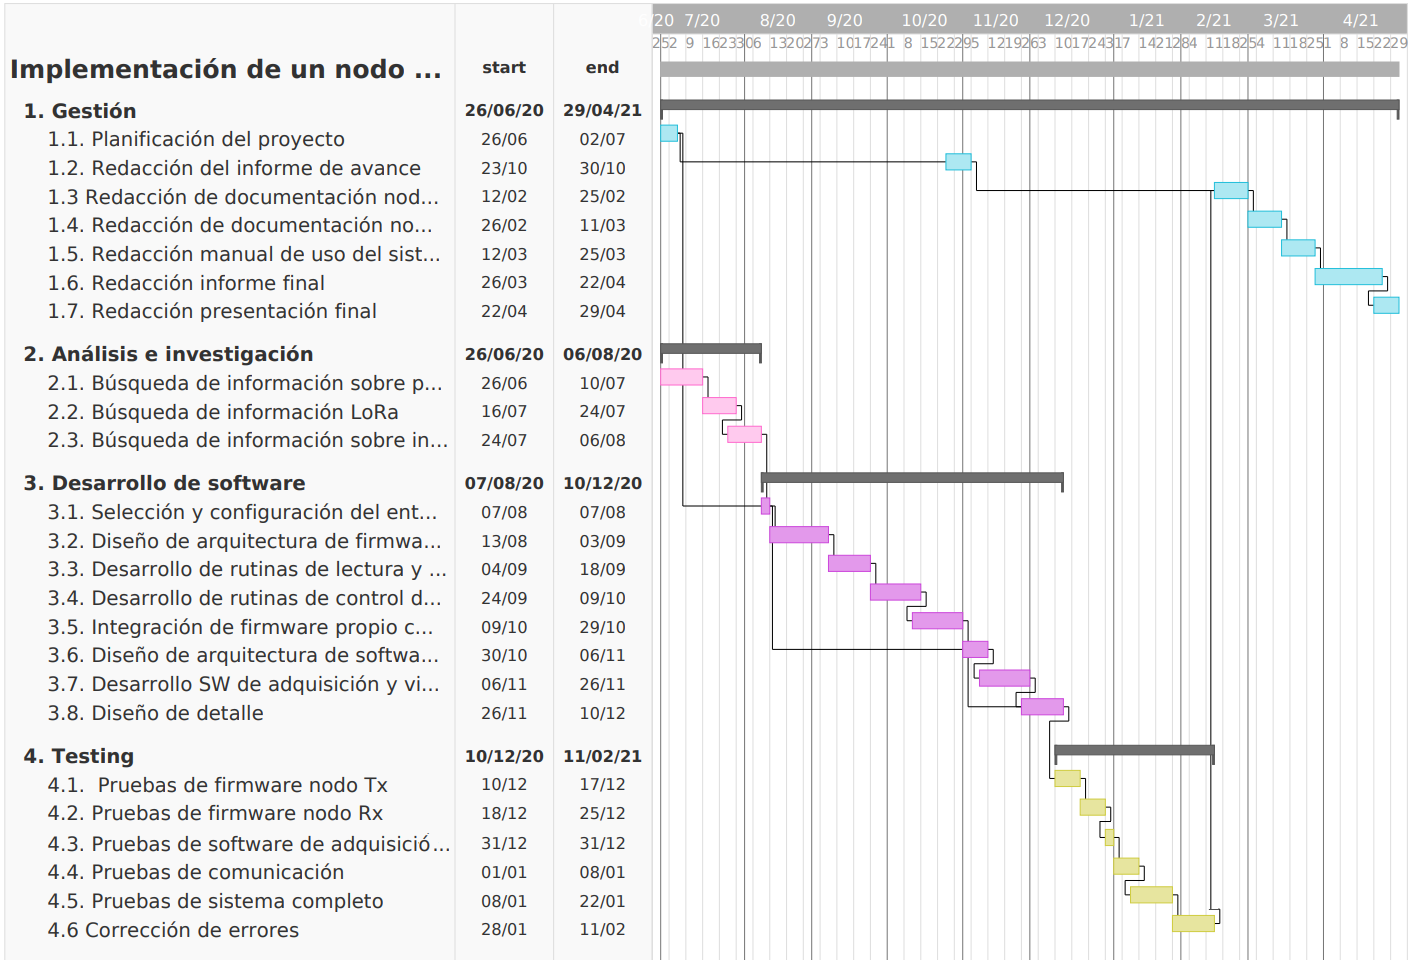
\includegraphics[width=1.5\textheight]{./Figuras/gantt.png}
\caption{Diagrama en \textit{Diagrama de Gantt del proyecto}}
\label{fig:Gantt}
\end{figure}
\end{landscape}
\section{9. Matriz de uso de recursos de materiales}
\label{sec:recursos}


\begin{table}[htbp]
\centering
\begin{tabularx}{\linewidth}{|c|X|c|c|c|c|}
\hline
\cellcolor[HTML]{C0C0C0}                                                                       & \cellcolor[HTML]{C0C0C0}                                                                            & \multicolumn{4}{c|}{\cellcolor[HTML]{C0C0C0}Recursos requeridos (horas)} \\ \cline{3-6} 
\multirow{-2}{*}{\cellcolor[HTML]{C0C0C0}\begin{tabular}[c]{@{}c@{}}Código\\ WBS\end{tabular}} & \multirow{-2}{*}{\cellcolor[HTML]{C0C0C0}\begin{tabular}[c]{@{}c@{}}Nombre\\ de tarea\end{tabular}} & PC       & Placas de desarrollo      & Sensores      & Raspberry Pi      \\ \hline
1.                                                                                             & Gestión                                                                                             & 190      &                           &               &                   \\ \hline
2.                                                                                             & Análisis e investigación                                                                            & 70       &                           &               &                   \\ \hline
3.                                                                                             & Desarrollo de software                                                                              & 230      & 100                       & 100           & 40                \\ \hline
4.1.                                                                                           & Pruebas de firmware de nodo transmisor                                                              &          & 20                        & 20            &                   \\ \hline
4.2.                                                                                           & Pruebas de firmware de nodo receptor                                                                &          & 20                        & 20            & 20                \\ \hline
4.3.                                                                                           & Pruebas de software de adquisición y visualización                                                  &          &                           &               & 10                \\ \hline
4.4.                                                                                           & Pruebas de comunicacion                                                                             &          & 20                        & 20            & 20                \\ \hline
4.5.                                                                                           & Pruebas de sistema completo                                                                         &          & 30                        & 30            & 30                \\ \hline
4.6.                                                                                           & Corrección de errores                                                                               & 40       & 40                        & 40            & 40                \\ \hline
\end{tabularx}
\end{table}


\section{10. Presupuesto detallado del proyecto}
\label{sec:presupuesto}

\begin{table}[htbp]
\begin{tabular}{|c|c|c|c|c|}
\hline
\rowcolor[HTML]{C0C0C0} 
Categoría         & Detalle               & Cantidad & Costo unitario (ARS) & Costo (ARS) \\ \hline
Costos directos   & Horas de ingeniería   & 630      & 400                  & 252000      \\ \hline
Costos indirectos & 30 \% costos directos & -        & -                    & 75600       \\ \hline
\multicolumn{4}{|c|}{\textbf{Total costos del proyecto}}                    & 3276000     \\ \hline
\end{tabular}
\end{table}

\section{11. Matriz de asignación de responsabilidades}
\label{sec:responsabilidades}

\begin{table}[htbp]
\begin{tabular}{|c|c|c|c|c|}
\hline
\rowcolor[HTML]{C0C0C0} 
\cellcolor[HTML]{C0C0C0}                                                                       & \cellcolor[HTML]{C0C0C0}                                     & \multicolumn{3}{c|}{\cellcolor[HTML]{C0C0C0}Listar todos los nombres y roles del proyecto}                                                                                                                                                      \\ \cline{3-5} 
\rowcolor[HTML]{C0C0C0} 
\multirow{-2}{*}{\cellcolor[HTML]{C0C0C0}\begin{tabular}[c]{@{}c@{}}Código\\ WBS\end{tabular}} & \multirow{-2}{*}{\cellcolor[HTML]{C0C0C0}Nombre de la tarea} & \begin{tabular}[c]{@{}c@{}}Responsable\\ \authorname\end{tabular} & \begin{tabular}[c]{@{}c@{}}Orientador\\ \supname\end{tabular} & \begin{tabular}[c]{@{}c@{}}Cliente\\ \clientename\end{tabular} \\ \hline
1.                                                                                             & Gestión                                                      & P                                                                                & C,A                                                                          & C,A                                                                           \\ \hline
2.                                                                                             & Análisis e investigación                                     & P                                                                                & C                                                                            & I                                                                             \\ \hline
3.                                                                                             & Desarrollo de software                                       & P                                                                                & C,A                                                                          & A                                                                             \\ \hline
5.                                                                                             & Testing                                                      & P                                                                                & C                                                                            & A                                                                             \\ \hline
\end{tabular}
\end{table}

{\footnotesize
Referencias:
\begin{itemize}
	\item P = Responsabilidad Primaria
	\item S = Responsabilidad Secundaria
	\item A = Aprobación
	\item I = Informado
	\item C = Consultado
\end{itemize}
} %footnotesize


\section{12. Gestión de riesgos}
\label{sec:riesgos}

\begin{consigna}{red}
a) Identificación de los riesgos (al menos cinco) y estimación de sus consecuencias:
 
Riesgo 1: detallar el riesgo (riesgo es algo que si ocurre altera los planes previstos)
\begin{itemize}
\item Severidad (S): mientras más severo, más alto es el número (usar números del 1 al 10).\\
Justificar el motivo por el cual se asigna determinado número de severidad (S).
\item Probabilidad de ocurrencia (O): mientras más probable, más alto es el número (usar del 1 al 10).\\
Justificar el motivo por el cual se asigna determinado número de (O). 
\end{itemize}   

Riesgo 2:
\begin{itemize}
\item Severidad (S): 
\item Ocurrencia (O):
\end{itemize}

Riesgo 3:
\begin{itemize}
\item Severidad (S): 
\item Ocurrencia (O):
\end{itemize}


b) Tabla de gestión de riesgos:      (El RPN se calcula como RPN=SxO)

\begin{table}[htpb]
\centering
\begin{tabularx}{\linewidth}{@{}|X|c|c|c|c|c|c|@{}}
\hline
\rowcolor[HTML]{C0C0C0} 
Riesgo & S & O & RPN & S* & O* & RPN* \\ \hline
       &   &   &     &    &    &      \\ \hline
       &   &   &     &    &    &      \\ \hline
       &   &   &     &    &    &      \\ \hline
       &   &   &     &    &    &      \\ \hline
       &   &   &     &    &    &      \\ \hline
\end{tabularx}%
\end{table}

Criterio adoptado: 
Se tomarán medidas de mitigación en los riesgos cuyos números de RPN sean mayores a ....

Nota: los valores marcados con (*) en la tabla corresponden luego de haber aplicado la mitigación.

c) Plan de mitigación de los riesgos que originalmente excedían el RPN máximo establecido:
 
Riesgo 1: Plan de mitigación (si por el RPN fuera necesario elaborar un plan de mitigación).
  Nueva asignación de S y O, con su respectiva justificación:
  - Severidad (S): mientras más severo, más alto es el número (usar números del 1 al 10).
          Justificar el motivo por el cual se asigna determinado número de severidad (S).
  - Probabilidad de ocurrencia (O): mientras más probable, más alto es el número (usar del 1 al 10).
          Justificar el motivo por el cual se asigna determinado número de (O).

Riesgo 2: Plan de mitigación (si por el RPN fuera necesario elaborar un plan de mitigación).
 
Riesgo 3: Plan de mitigación (si por el RPN fuera necesario elaborar un plan de mitigación)

\end{consigna}


\section{13. Gestión de la calidad}
\label{sec:calidad}

\begin{consigna}{red}
Para cada uno de los requerimientos del proyecto indique:
\begin{itemize} 
\item Req \#1: Copiar acá el requerimiento.

Verificación y validación:

\begin{itemize}
\item Verificación para confirmar si se cumplió con lo requerido antes de mostrar el sistema al cliente:\\
Detallar 
\item Validación con el cliente para confirmar que está de acuerdo en que se cumplió con lo requerido:\\
Detallar  
\end{itemize}

\end{itemize}

Tener en cuenta que en este contexto se pueden mencionar simulaciones, cálculos, revisión de hojas de datos, consulta con expertos, etc.

\end{consigna}

\section{14. Comunicación del proyecto}
\label{sec:comunicaciones}

\begin{consigna}{red}
El plan de comunicación del proyecto es el siguiente:
\end{consigna}

% Please add the following required packages to your document preamble:
% \usepackage{graphicx}
% \usepackage[table,xcdraw]{xcolor}
% If you use beamer only pass "xcolor=table" option, i.e. \documentclass[xcolor=table]{beamer}
\begin{table}[htpb]
\centering
\resizebox{\textwidth}{!}{%
\begin{tabular}{|c|c|c|c|c|c|}
\hline
\rowcolor[HTML]{C0C0C0} 
\multicolumn{6}{|c|}{\cellcolor[HTML]{C0C0C0}PLAN DE COMUNICACIÓN DEL PROYECTO}           \\ \hline
\rowcolor[HTML]{C0C0C0} 
¿Qué comunicar? & Audiencia & Propósito & Frecuencia & Método de comunicac. & Responsable \\ \hline
                &           &           &            &                      &             \\ \hline
                &           &           &            &                      &             \\ \hline
                &           &           &            &                      &             \\ \hline
                &           &           &            &                      &             \\ \hline
                &           &           &            &                      &             \\ \hline
\end{tabular}%
}
\end{table}

\section{15. Gestión de compras}
\label{sec:compras}

\begin{consigna}{red}
En caso de tener que comprar elementos o contratar servicios:
a) Explique con qué criterios elegiría a un proveedor.
b) Redacte el Statement of Work correspondiente.
\end{consigna}

\section{16. Seguimiento y control}
\label{sec:seguimiento}

\begin{consigna}{red}
Para cada tarea del proyecto establecer la frecuencia y los indicadores con los se seguirá su avance y quién será el responsable de hacer dicho seguimiento y a quién debe comunicarse la situación (en concordancia con el Plan de Comunicación del proyecto).

El indicador de avance tiene que ser algo medible, mejor incluso si se puede medir en \% de avance. Por ejemplo,se pueden indicar en esta columna cosas como ``cantidad de conexiones ruteadeas'' o ``cantidad de funciones implementadas'', pero no algo genérico y ambiguo como ``\%'', porque el lector no sabe porcentaje de qué cosa.

\end{consigna}

\begin{table}[!htpb]
\centering
\begin{tabularx}{\linewidth}{@{}|X|X|X|X|X|X|@{}}
\hline
\rowcolor[HTML]{C0C0C0} 
\multicolumn{6}{|c|}{\cellcolor[HTML]{C0C0C0}SEGUIMIENTO DE AVANCE}                                                                       \\ \hline
\rowcolor[HTML]{C0C0C0} 
Tarea del WBS & Indicador de avance & Frecuencia de reporte & Resp. de seguimiento & Persona a ser informada & Método de comunic. \\ \hline
 &  &  &  &  &  \\ \hline
 &  &  &  &  &  \\ \hline
 &  &  &  &  &  \\ \hline
 &  &  &  &  &  \\ \hline
 &  &  &  &  &  \\ \hline
\end{tabularx}%
%}
\end{table}

\section{17. Procesos de cierre}    
\label{sec:cierre}

\begin{consigna}{red}
Establecer las pautas de trabajo para realizar una reunión final de evaluación del proyecto, tal que contemple las siguientes actividades:

\begin{itemize}
\item Pautas de trabajo que se seguirán para analizar si se respetó el Plan de Proyecto original:
 - Indicar quién se ocupará de hacer esto y cuál será el procedimiento a aplicar. 
\item Identificación de las técnicas y procedimientos útiles e inútiles que se utilizaron, y los problemas que surgieron y cómo se solucionaron:
 - Indicar quién se ocupará de hacer esto y cuál será el procedimiento para dejar registro.
\item Indicar quién organizará el acto de agradecimiento a todos los interesados, y en especial al equipo de trabajo y colaboradores:
  - Indicar esto y quién financiará los gastos correspondientes.
\end{itemize}

\end{consigna}


\end{document}
